\chapter{Development}\label{ch:development}
\section{Component List}
\subsection{Introduction}
To create the basis for development of this project two microphones and a structure to keep a constant distance between them were necessary.  

\subsection{Microphones characteristics}
\paragraph{}
Firstly a decision had to be made whether to use a directional or omnidirectional microphone. Since omnidirectional microphones provide less plosive and wind sounds, does not build up bass it was considered a good option. The fact that it provides equally good audio quality at every angle made it the best choice for the aim of this project.

Voice frequency ranges vary heavily depending on whether it sources from a male of a female. Fundamental voice frequency varies from 100Hz to 900 Hz for men and 350Hz to 3KHz for women. Including peaks to conserve natural sounding voice, a wider frequency range has to be considered. It rises to 8 KHz for males and 17KHz for females \cite{Seaindia}. Yet different researches often come up with different results. For example, in phone communications it is accepted to transmit frequency range between 400Hz and 3400Hz. This is the reason some peoples' voices transit poorly over the phone yet for most cases it works fine. This example allows to conclude that smaller frequency ranges could be acceptable but to conserve all of the properties of the human voice microphones do need to be capable of recording at 17kHz. 
\paragraph{Our requirements for the microphones were: \\}

\paragraph{• Affordable price\\}   
Since the university did not have any planned funding for this semester, it was agreed to aim for budget options. This way it would not be necessary to work towards an agreement with the University to receive funding - some members wanted to have microphones for themselves.
\paragraph{• Capability to capture the entire range of human hearing frequency\\}   
Since one of the great benefits of an omnidirectional microphone was it's ability to capture clear sound, it would not have been reasonable to purchase microphones that were not able to capture the full clarity of the input. Since the entire human voice frequency fits within our hearing frequency range, there is no need to have any extra requirements.
\paragraph{• Appropriate size factor\\}    
It would be beneficial and logical if the microphones used in the testing would have potential to be a part of the design prototype. Although due to limited budget there is a low chance of affording the microphones with an appropriate size parameters for a hearing aid or earphones, objective to apply a microphone that could be used in the further stages of development remains as one of lower priorities    
\paragraph{• They must to be identical\\}    
Having identical microphones assures that if there was a delay within recording timings, it would not be caused by hardware differences.
\paragraph{• Capability to connect multiple microphones to a single computer and record both at the same time\\}   
For the sake of simplicity regarding sampling and testing, it was agreed that it would be far easier to sample using microphones that can be connected though Universal Serial Bus port instead of Auxiliary one. This way troubleshooting and initiating microphones should be more clear. 

\subsection{Microphones}
As requirements for microphones were set, it was first attempted to find them at the University. As it was found that University does not own any microphones that could be applied for the purpose of this project, it was agreed to purchase budget microphones that could come as close to the requirements raised for the project as possible. Bearing in mind that a month-long delivery from Asia is not a viable option, it was decided to order microphones available within an acceptable delivery time \todo{ microphone reference}.\\

\subsection{Distancing}
To maintain a constant distance it was decided to attempt modeling a rod with two microphone holders at it's ends. The distance chosen between the microphones was agreed on by referring to a research article in this area: 15.2 centimeters \todo{reference}. 
\paragraph{}
Other parameters were found by following the measurements found in the datasheet \ref{fig:MicData}. These steps have led us towards the structure development, which after a few iterations has turned into the structure that was used for sampling \todo{illustration missing (3D model or real one)}.
\begin{figure} [htp] 
  \centering
    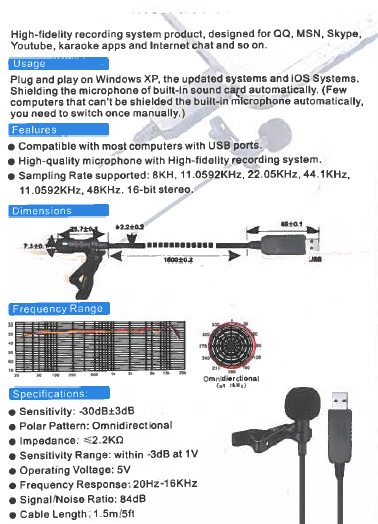
\includegraphics[width=0.5\textwidth]{Illustrations/MicData}
    \caption{Microphones data sheet}
    \label{fig:MicData}
\end{figure}

\todo[inline,color=green]{\url{https://www.researchgate.net/publication/228749231_Analysis_of_the_Facial_Anthropometric_Data_of_Korean_Pilots_for_Oxygen_Mask_Design}}

\section{Setting up the scene}
Sampling was done in a lecture/ conference room with side noise: a server, maintaining the virtual conference platform (B107). This area was chosen because it had represented a real life conversation scenario. It is planned to conduct tests with a working system in a different environments to validate the effectiveness of it. Creating a set of samples in every different environment throughout the development phase would take a lot of time and therefore was considered unnecessary for the early stages. 
\paragraph{}
Since the sampling ratio of human ear can only reach up to 20kHz, 48kHz sampling frequency of the microphones the Nyquist frequency and therefore guarantees that there will not be any hearable audio quality losses.   
\subsection{Analog to digital conversion}
Since the datasheet of the microphone does not provide any information on the Analog-to-Digital Converter that is used to process the data and there is not default ADC that is used for this process, the only potentially successful way to find the details about the ADC used for the signal processing is to open the microphone and look for the information on the ADC itself. Since the structure seemed to be glued together, we will not attempt to find the details of it and just rely on the specifications sheet provided by the manufacturer.  

 

